% This program can be redistributed and/or modified under the terms
% of the GNU Public License, version 3.
%
% Seth Brown, Ph.D.
% sethbrown@drbunsen.org
%
% Compiled with XeLaTeX
% Dependencies:
%   Fontin Sans font (http://www.exljbris.com/fontinsans.html)
%

% TODO: Add citations as bibtex

\documentclass[unknownkeysallowed]{beamer}

\usepackage{graphicx} % graphics
\usepackage{epsfig} % eps graphics
\usepackage{hyperref} % urls
\usepackage{booktabs, caption} % table styling

% suppress navigation bar
\beamertemplatenavigationsymbolsempty

\mode<presentation>
{
  \usetheme{bunsen}
  \setbeamercovered{transparent}
  \setbeamertemplate{items}[circle]
}

% set fonts
\usepackage{fontspec}
\setsansfont{Fontin Sans}
\setbeamerfont{frametitle}{size=\LARGE,series=\bfseries}

% color definitions
\usepackage{color}
\definecolor{uipoppy}{RGB}{225, 64, 5}
\definecolor{uipaleblue}{RGB}{96,123,139}
\definecolor{uiblack}{RGB}{0, 0, 0}

% caption styling
\DeclareCaptionFont{uiblack}{\color{uiblack}}
\DeclareCaptionFont{uipoppy}{\color{uipoppy}}
\captionsetup{labelfont={uipoppy},textfont=uiblack}

% see the macros.tex file for definitions
% This program can be redistributed and/or modified under the terms
% of the GNU Public License, version 3.

% adds reference to bottom right of corner of a slide
\usepackage[absolute,overlay]{textpos} % text references in slide corners
\newcommand\textref[1]{%
  \begin{textblock*}{\paperwidth}(0pt,0.99\textheight)
  \raggedleft \tiny{\emph{#1}}\hspace{.5em}
  \end{textblock*}}

% for drawing circles around numbers
% ex. \circled{1} Add some text here.
\usepackage{tikz}
\newcommand*\circled[1]{\tikz[baseline=(char.base)]{
            \node[shape=circle,draw,inner sep=2pt] (char) {#1};}}


% title slide definition
\title{Get Git}
\author{Chris Keefe}
\institute{Northern Arizona University \\
Department of Computer Science \\
School of Informatics, Computing, and Cyber Systems \\
}

\date{\today}

%--------------------------------------------------------------------
%                           Introduction
%--------------------------------------------------------------------

\begin{document}

\section{Introduction}
\setbeamertemplate{background}
{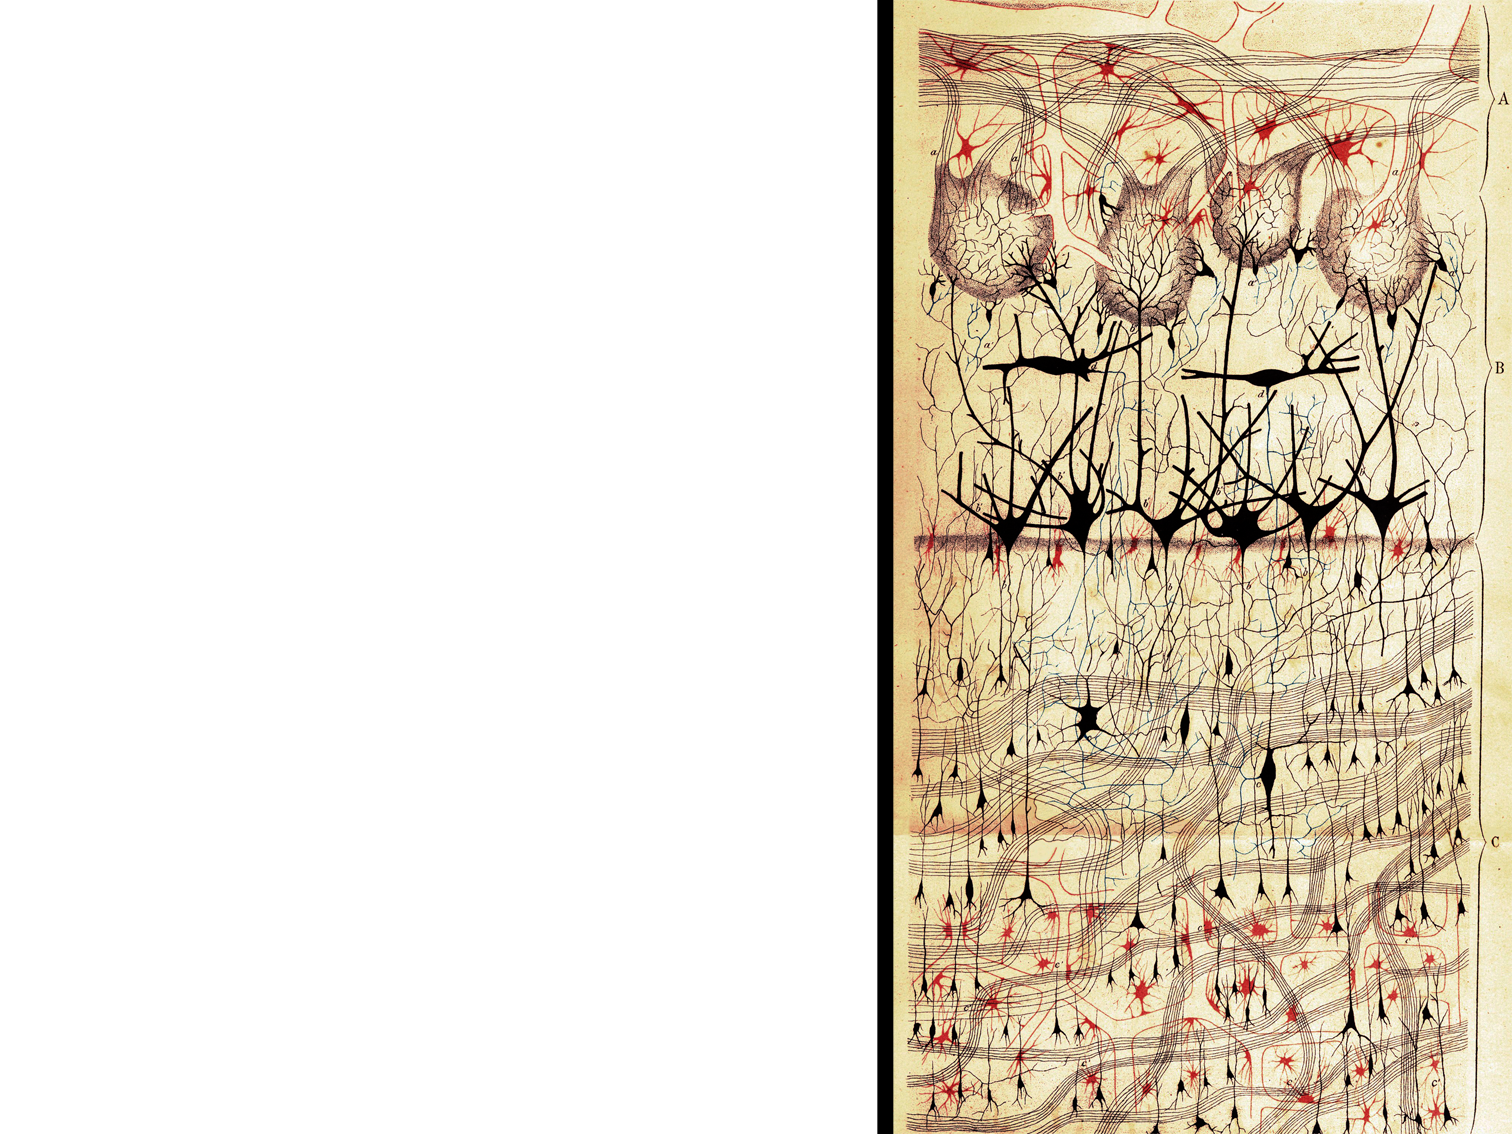
\includegraphics[width=\paperwidth,height=\paperheight]{assets/frontpage_bg}}
\setbeamertemplate{footline}[default]

\begin{frame}
\vspace{2cm}
\begin{columns}
\column{2.75in}
  \titlepage
  \vspace{10cm}
\column{2.0in}
\end{columns}
\end{frame}

%-------------------------------------------------------------------
%                          Section 1
%-------------------------------------------------------------------
%
% Set the background for the rest of the slides.
% Insert infoline
\setbeamertemplate{background}
 {
\includegraphics[width=\paperwidth,height=\paperheight]{assets/slide_bg}}
\setbeamertemplate{footline}[bunsentheme]

\section{What, Why, and How?}
\begin{frame}
    \frametitle{What is git?}

    \vspace{1cm} % generate some space between title and content
    \begin{table}[h]
    \centering
    \begin{tabular}{lcccc} \bottomrule[2pt]
        Name & Symbol & $A_r$ & M.P. (K) & IE (J) \\ \bottomrule
        Helium & He & $4.00$ & $1$ & $3.94e^{-18}$ \\
        Carbon & C & $12.01$ & $773$ & $3.94e^{-18}$ \\
        Arsenic & As & $74.92$ & $1090$ & $1.48e^{-18}$ \\
        Gold & Au & $196.96$ & $1337$ & $1.48e^{-18}$ \\
        Cobalt & Co & $58.93$ & $1495$ & $1.26e^{-18}$ \\
    \bottomrule[2pt]
    \end{tabular}
    \caption{Properties of Whoville Elements}
    \end{table}

    \vspace{-0.6cm} % compact spacing between table and text

    \begin{columns}[t]
    \column{4.5cm}
    \begin{block}{Trace rare earth metals:}
    \begin{itemize}
        \item{Ytterbium}
        \item{Neodymium}
        \item{Praseodymium}
    \end{itemize}
    \end{block}
    \column{4.5cm}
    \begin{block}{Obtaining Neodymium:}
        \vspace{0.15cm}
        \circled{1}$\textemdash$bastn\"{a}site \\
        \circled{2}$\textemdash${monazite} \\
    \end{block}
    \end{columns}

\end{frame}

\begin{frame}
    \frametitle{Git is not GitHub}
    \vspace{1cm} % generate some space between title and content
\end{frame}

\begin{frame}
    \frametitle{Who uses git?}

    \vspace{1cm} % generate some space between title and content
\end{frame}

\begin{frame}
    \frametitle{Why do I use git?}
    \begin{itemize}
        \item{It's required by my job.}
        \item{Alongside GitHub, git makes showing off easy.}
        \item{It gives me fast, free, highly redundant version control.}
        \item{It makes it easier to work with other people.}
        \item{It makes contributing to open source much easier.}
    \end{itemize}
    \vspace{1cm} % generate some space between title and content
\end{frame}

\begin{frame}
    \frametitle{Git and Operating Systems}
    \begin{itemize}
        \item{Windows doesn't git well.}
        \item{Linux install through package manager}
        \item{Mac: ???}
    \end{itemize}
    \vspace{1cm} % generate some space between title and content
\end{frame}

\begin{frame}
    \frametitle{Git and Operating Systems}
    \begin{itemize}
        \item{Windows doesn't git well.}
        \item{Linux install through package manager}
        \item{Mac: ???}
    \end{itemize}
    \vspace{1cm} % generate some space between title and content
\end{frame}
\section{Getting Started with git}

\begin{frame}
    \frametitle{Our Sample Workflow}
      Simple graphic displaying our workflow with labels for
      \begin{itemize}
        \item{working dir}
        \item{local repo}
        \item{origin repo}
        \item{upstream repo}
      \end{itemize}
    \vspace{1cm} % generate some space between title and content
\end{frame}

\begin{frame}
    \frametitle{Get source code}
    \begin{itemize}
        \item{sign up for hacktoberfest}
        \item{Fork the repo to which you want to contribute}
        \item{Clone the repo - copies it to your local machine.  ``` git clone <repo html>```}
        \item{Mac: ???}
    \end{itemize}
    \vspace{1cm} % generate some space between title and content
\end{frame}

\end{document}

